\documentclass{vgtc}

% set font encoding for PDFLaTeX or XeLaTeX
\usepackage{ifxetex}
\ifxetex
  \usepackage{fontspec}
\else
  \usepackage[T1]{fontenc}
  \usepackage[utf8]{inputenc}
  \usepackage{lmodern}
\fi
\usepackage{graphicx}
\usepackage{float}
\usepackage{cite}

% used in maketitle
\title{Study of freight accross Europe.}
\author{Barbier Jeremy, Bazin Adelme, Paffoni Nina}


\begin{document}
\maketitle

\section{Introduction}
In a world always more globalized, we found interesting to produce visualization about the transports of goods around the world. Our work is intended for people that want to know more about the freight between countries. The goal of this work is to highlight which countries are the biggest importers, which are the biggest exporters, and between which there are the most exchanges. 
Another purpose of this project is to show this data considering the year studied. The target audience for this type of visualization will be anyone who wants to see the evolution of the world’s freight, and maybe correlate it with such-and-such element (for example a political change, maybe on the environmental policy). 

To have something visual for the user, we choose to make an interactive map of Europe. This article will first describe the state of the art, and then discuss in what our visualization will be useful. The data the will be used will also be described. 

\section{Related Work}
An intuitive visualisation is proposed on the shipmap.org website \cite{shipmap} which focuses on maritime transports around the world. Each ship is represented by a dot of different colour according to the type of ship (Container, Tanker, Vehicle…). It looks like (at a larger scale) what we want to produce, but with some inconvenients. First, the type of goods is not detailed, because of the use of colours, which restrains the different representable types to a small number if we want to keep simplicity. Finally, there is no indication about the quantity of goods transported by each ship, so we don’t have information on the proportions of goods sent or received by each country. In this case, we don’t have the information on the quantity of goods that the ship carrying.

\begin{figure}[H]
\center
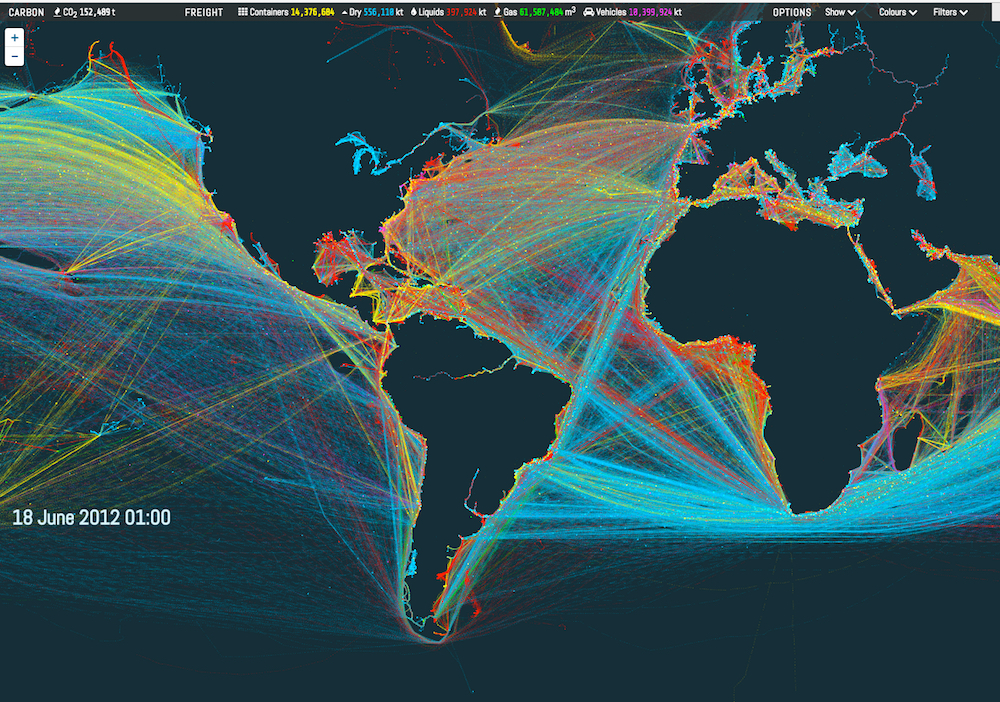
\includegraphics[scale=0.2]{shipmap.jpg}
\end{figure}

Furthermore, we’d like to keep the idea of a map as a function of time, to show the evolution of freight in UE for several years (depending on what is shown/the data used). 

Concerning network visualization, which we want to produce to show exchange between countries, we will base our work on visualizations produced by Martin Grandjean \cite{airtraffic}. This visualization is really good to show the principal localisation for the freight but it is way too complex to allow us to show the type of goods, or to differentiate importation and exportation. So we’ll have to simplify it before adding what we want to show in our visualization.

\begin{figure}[H]
\center
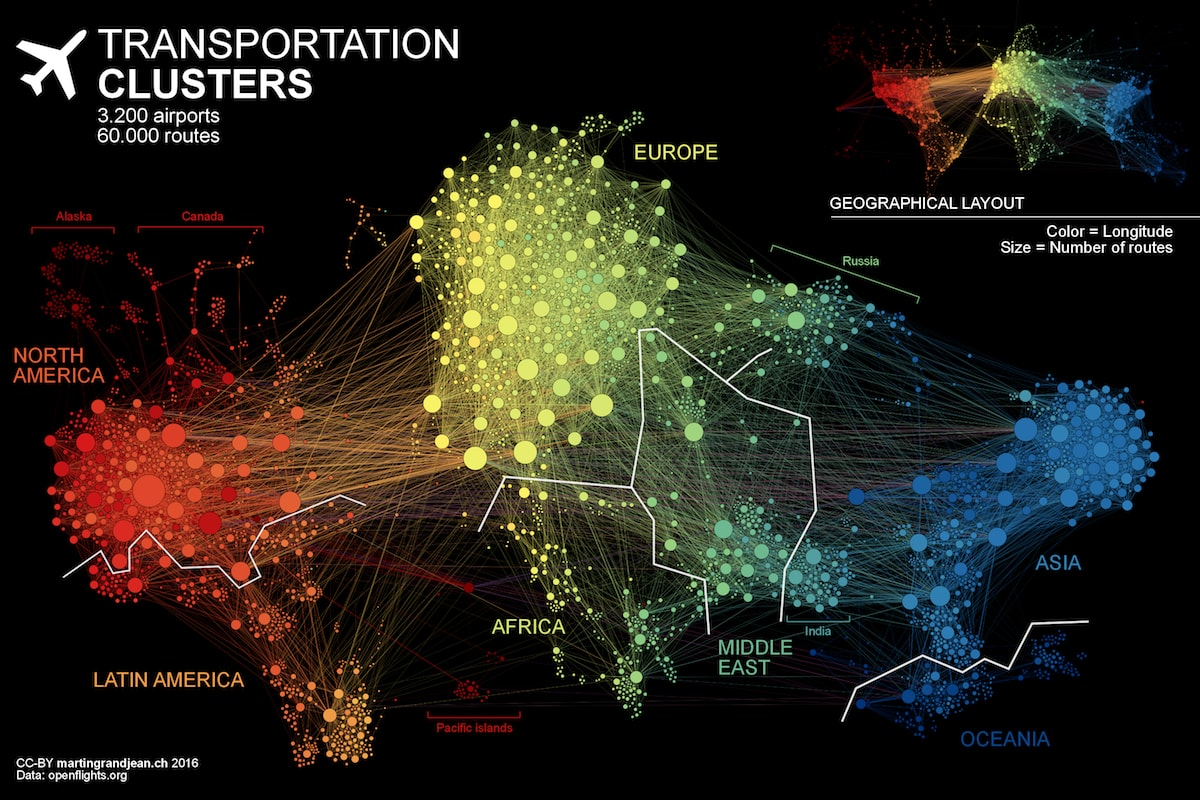
\includegraphics[scale=0.15]{airports-network-small.jpg}
\end{figure}

This third example of vizualisation shows another network. It’s presented in the atlas of economic complexity \cite{atlas}. Each node represents a product. It enables to present multiples products at once, but there is a single visualization for each country so it can be difficult if we want to compare countries between each other.

\begin{figure}[H]
\center
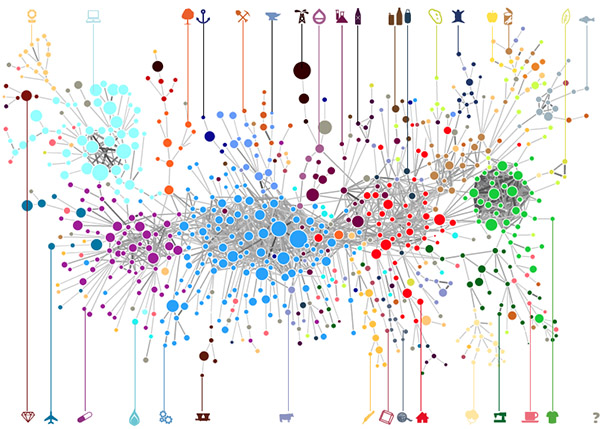
\includegraphics[scale=0.4]{economic_growth_atlas2.jpg}
\end{figure}

We decided to limit ourselves to the UE area and to focus on road freight, to keep the visualization simple by not adding too much information on it. Our work will be based on the one already done by the Eurostat organism, which has collected data about road, rail, sea and air freight in the European union. We will first focus on road freight (which represents about 75\% of the european freight \cite{dataset}), and eventually add rail if possible.

Bar chart visualization have already been made by Eurostat, to show for example the repartition of type of transport for each country for a particular year. However we did not found any map visualization that could summarize the data. Plus we did not found in this work any visualization concerning the exchanges between countries.

\section{Design Visualisation}
We chose to start from maps to consider geographical advantages and constraints of each countries. This visualization gives a global point of view and it is very easy to understand by anyone. It appeared to us that it was primordial to keep simplicity that’s why we will also exclude representing imports and exports in the same visualisation to avoid overloading.
The map offers global visualization but we want to allow the user to have more details by interacting with the visualization. For example by clicking on a specific country the user will show informations on types of goods.
We want to use interactivity to keep visualization simple whichever level of detail is displayed.
We’ll represent the evolution through time to show changes. We could use a cursor and/or an automatic display of time.

\begin{figure}[H]
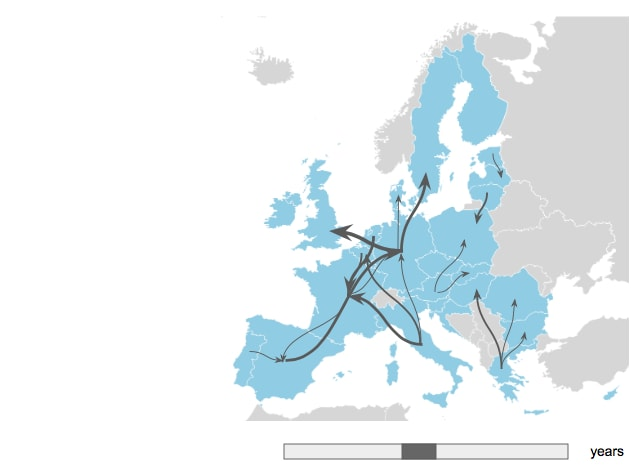
\includegraphics[scale=0.35]{Capture_ecran_2017-11-29_171310.jpg}
\caption{Proposition of global visualization, showing flow of freight across UE}
\end{figure}

\begin{figure}[H]
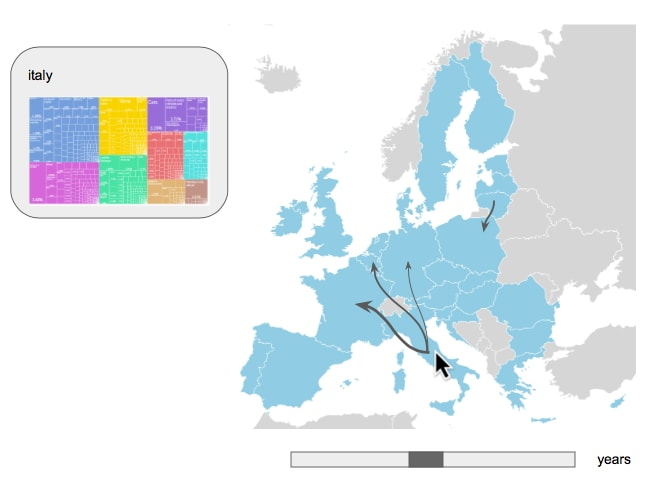
\includegraphics[scale=0.35]{Capture_ecran_2017-11-29_171255.jpg}
\caption{By clicking on a specific country (here Italy), the user will see only the flow of goods that involve the country and display details concerning types of goods}
\end{figure}

\section{Conclusion \& Perspectives}
As mentionned in the related work, our topic has already a lot of different visualizations. But it is also a complex theme, and it seems to lack of global visualization offering an overview of the european freight. So we will try to make one that allows the user to easily identify differences between countries for the quantity of goods imported/exported. It will also bring more detailed informations if the user wants to, by clicking on the country of interest. Finally, we’d like to allow the user to study the impact of a change that happened at a certain time, by providing a navigation trough time for the visualization.
\bibliographystyle{plain}
\bibliography{template}
\end{document}
